\scanpage{30}\mspage{29}
% @ top, proposition heading
\uline{Proposition} Let $F',F,G$ be three figures.
% @ top, three implications
\[
\begin{aligned}
 \text{a)}\quad F'\ll F&\Longrightarrow F'.G\ll F.G\\
 \text{b)}\quad F'\preceq F&\Longrightarrow F'.G\preceq F.G\\
 \text{c)}\quad F'\leq F&\Longrightarrow F'.G\leq F.G\quad{}^{*}
\end{aligned}
\]
% @ upper right, beside a
\margin{(trivial by definition of $\ll$ as Inf)}
% @ upper right, beside b
\margin{(\unsure{follows} from a), by looking at supports)}
% @ upper left, starred gloss
\margin{$*$ \uline{\unsure{making explicit|explanation}}}
% @ upper part, starred formula
\[
 F'.G=\{A\in F.G\mid A\subset |F'|\}
\]

% @ upper part, proof lines 1–2
Let us prove c. We must prove that \deleted{$F'.G$} $F'.G\subset F.G$, and is closed in $F.G$.

% @ middle, proof lines 1–5
\deleted{\unsure{now|these|this}} Now $F'.G$ is formed of the $A\cap B$ $(A\in F',B\in G)$ such that $A^\circ\cap B^\circ\ne\phi$, and $F.G$ of the $A\cap B$ $(A\in F,B\in \unsure{G|L})$ such that $A^\circ\cap B^\circ\ne\phi$, and in both cases \unsure{the|the} meaning of $A^\circ$ (with respect to $F$, \unsure{in|in} $F'$) is the same, hence $F'.G\subset F.G$. Let us prove that it is closed i.e.
% @ center, first membership and annotations
If \deleted{$(\deleted{A\cap B}\qquad A,A'\in F',$}
\[
 \underset{\substack{\rotatebox{-90}{$\in$}\\ F'}}{A}\cap
 \underset{\substack{\rotatebox{-90}{$\in$}\\ G}}{B}\in F'.G\qquad
 \text{i.e. } A^\circ\cap B^\circ\ne\phi
\]
% @ center, second membership and annotations
\figure{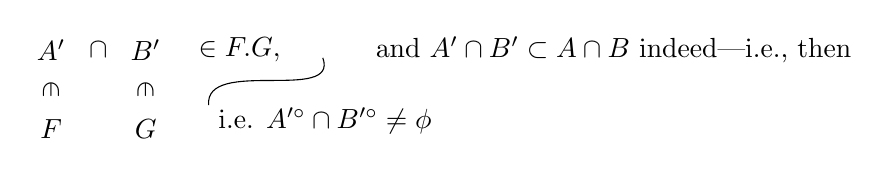
\begin{tikzpicture}[x=1cm,y=1cm]
\node at (0,0) {$A'$};
\node at (.6,0) {$\cap$};
\node at (1.2,0) {$B'$};
\node[anchor=west] at (1.75,0) {$\in F.G,$};
\node[rotate=-90] at (0,-.5) {$\in$};
\node[rotate=-90] at (1.2,-.5) {$\in$};
\node at (0,-1) {$F$};
\node at (1.2,-1) {$G$};
\node[anchor=west] at (4,0) {and $A'\cap B'\subset A\cap B$ \deleted{\unsure{indeed|i.e.}}, then};
\node[anchor=west] (ins) at (2,-.9) {\inserted{i.e. $A'^\circ\cap B'^\circ\ne\phi$}};
\draw (3.45,-.1) to[out=-70,in=95] (2,-.7);
\end{tikzpicture}}
% @ middle lower, conclusion lines 1–4
$A'\cap B'\in F'.G$ i.e. $A'\in F'$. Now we know that (according to the theory of $F.G$) that $A'\cap B'\subset A\cap B\Longrightarrow A'\subset A$, $B'\subset B$, whence $A'\in F'$ since $F'$ closed in $F$.

% @ lower left, oblique explanation
% slanted; source note rotated -45 degrees for inspection; final short label below the inverse-image line
\margin{\uline{Make explicit}~: let
\diagram{\begin{tikzcd}[ampersand replacement=\&,column sep=small,row sep=small]
 G\arrow[r,phantom,"\leq" description]\&F\arrow[d,phantom,"\rotatebox{90}{$\unsure{\preceq|\ll}$}" description]\\
 {}\&F'
\end{tikzcd}}, whence $G'$ \unsure{with} $G'\preceq G$, $G'\leq F'$. Then we have $G'=\{A'\in F'\mid A'\subset |G|\}=\varphi^{-1}(G)$, where $\varphi:F'\to F\ldots$ \unsure{$C_3$.|Corollary.|C6.}}
% @ lower right, note on uniqueness; two separate vertical grouping strokes on its left are reproduced
\margin{\figure{\begin{tikzpicture}
\node[anchor=north west,inner sep=0pt,text width=2.05cm] (uppernote) at (0,0) {A little hasty, we find by $F'.G=G'$ a $G'$ such that
\diagram{\begin{tikzcd}[ampersand replacement=\&,column sep=small,row sep=small]
 F'\arrow[r,phantom,"\preceq" description] \arrow[d,phantom,"\rotatebox{90}{$\leq$}" description]\& F\arrow[d,phantom,"\rotatebox{90}{$\leq$}" description]\\
 G'\arrow[r,phantom,"\preceq" description]\& G
\end{tikzcd}}
but we must still check \uline{uniqueness}};
\draw ([xshift=-4pt]uppernote.north west) -- ([xshift=-4pt,yshift=1pt]uppernote.south west);
\draw ([xshift=-1pt,yshift=-7pt]uppernote.north west) -- ([xshift=-1pt,yshift=-1pt]uppernote.south west);
\end{tikzpicture}}}
% @ lower right, second note; left boundary steps right after the first b line, then descends alongside its continuation
\margin{\figure{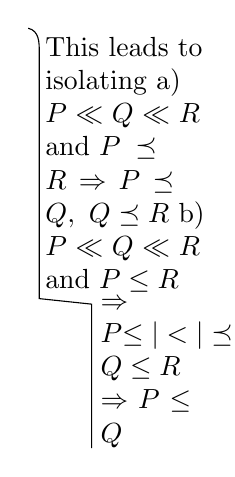
\begin{tikzpicture}
\node[anchor=north west,inner sep=0pt,text width=2.05cm] (lowernote) at (0,0) {This leads to isolating a) $P\ll Q\ll R$ and $P\preceq R\Rightarrow P\preceq Q,\ Q\preceq R$ b) $P\ll Q\ll R$ and $P\leq R$};
\node[anchor=north west,inner sep=0pt,text width=1.35cm] (continuation) at ([xshift=7mm,yshift=-2pt]lowernote.south west) {\deleted{$\Rightarrow P\unsure{\leq|<|\preceq}$} $Q\leq R$\\$\Rightarrow P\leq Q$};
\draw ([xshift=-6pt,yshift=3pt]lowernote.north west) .. controls ([xshift=-2pt,yshift=2pt]lowernote.north west) and ([xshift=-2pt,yshift=-2pt]lowernote.north west) .. ([xshift=-2pt,yshift=-6pt]lowernote.north west) -- ([xshift=-2pt,yshift=-2pt]lowernote.south west) -- ([xshift=-3pt,yshift=-2pt]continuation.north west) -- ([xshift=-3pt]continuation.south west);
\end{tikzpicture}}}
% @ lower part, corollary
\uline{Corollary.} The axiom C6 is valid.

% @ lower part, introduction to C7; small 0 is attached to the 7 in this main line, beside the right-note boundary
Let us check C7$_0$ all the same
% @ lower part, order diagram and existence
\diagram{\begin{tikzcd}[ampersand replacement=\&,column sep=small,row sep=small]
 G\arrow[r,phantom,"\leq" description]\arrow[d,phantom,"\rotatebox{90}{$\preceq$}" description]\&F\& {\exists\ \text{subdivision }F'\text{ of }F\text{ which}}\\
 G'\& {}\&{\text{induces }G'.}
\end{tikzcd}}
% @ bottom, construction
We take $F'=G'\cup\deleted{(\unsure{F\setminus G|F.G|F\times G}\unsure{2|?})}(F\setminus G)$ (disjoint union)
% @ bottom, verification items
We must check a) it is a figure b) that \deleted{\unsure{refines}}\inserted{subdivides} $F$ and c) which induces $G'$ on $G$.
